\chapter{Conception}
\clearpage

\section{Introduction}
La phase de conception constitue une étape déterminante dans le cycle de développement logiciel. 
Elle permet de traduire les besoins fonctionnels identifiés en une architecture technique cohérente. 
Cette étape définit non seulement l'architecture globale et les composants principaux du système, 
mais aussi les interactions entre les différents modules.

La conception du système OptiHR s'inscrit dans une démarche méthodique visant à garantir 
la qualité, la maintenabilité et l'évolutivité de la solution. Une attention particulière 
a été portée à la modélisation des données et à l'organisation des classes pour refléter 
fidèlement les processus métier de l'ARCOP.

\section{Architecture du système}

\subsection{Architecture globale}
Le système OptiHR adopte une architecture en couches qui permet une séparation claire des responsabilités:

\begin{itemize}
    \item \textbf{Couche Présentation}: Interfaces utilisateur accessibles via navigateur web, incluant les templates Blade, les feuilles de style CSS et le code JavaScript.
    \item \textbf{Couche Application}: Logique métier et traitement des requêtes via les contrôleurs Laravel et les services métier.
    \item \textbf{Couche Persistance}: Stockage et récupération des données à travers l'ORM Eloquent et la base de données PostgreSQL.
\end{itemize}

Cette architecture en trois couches favorise la modularité et facilite la maintenance du code en isolant 
les changements à des zones spécifiques du système.

\begin{figure}[H]
    \centering
    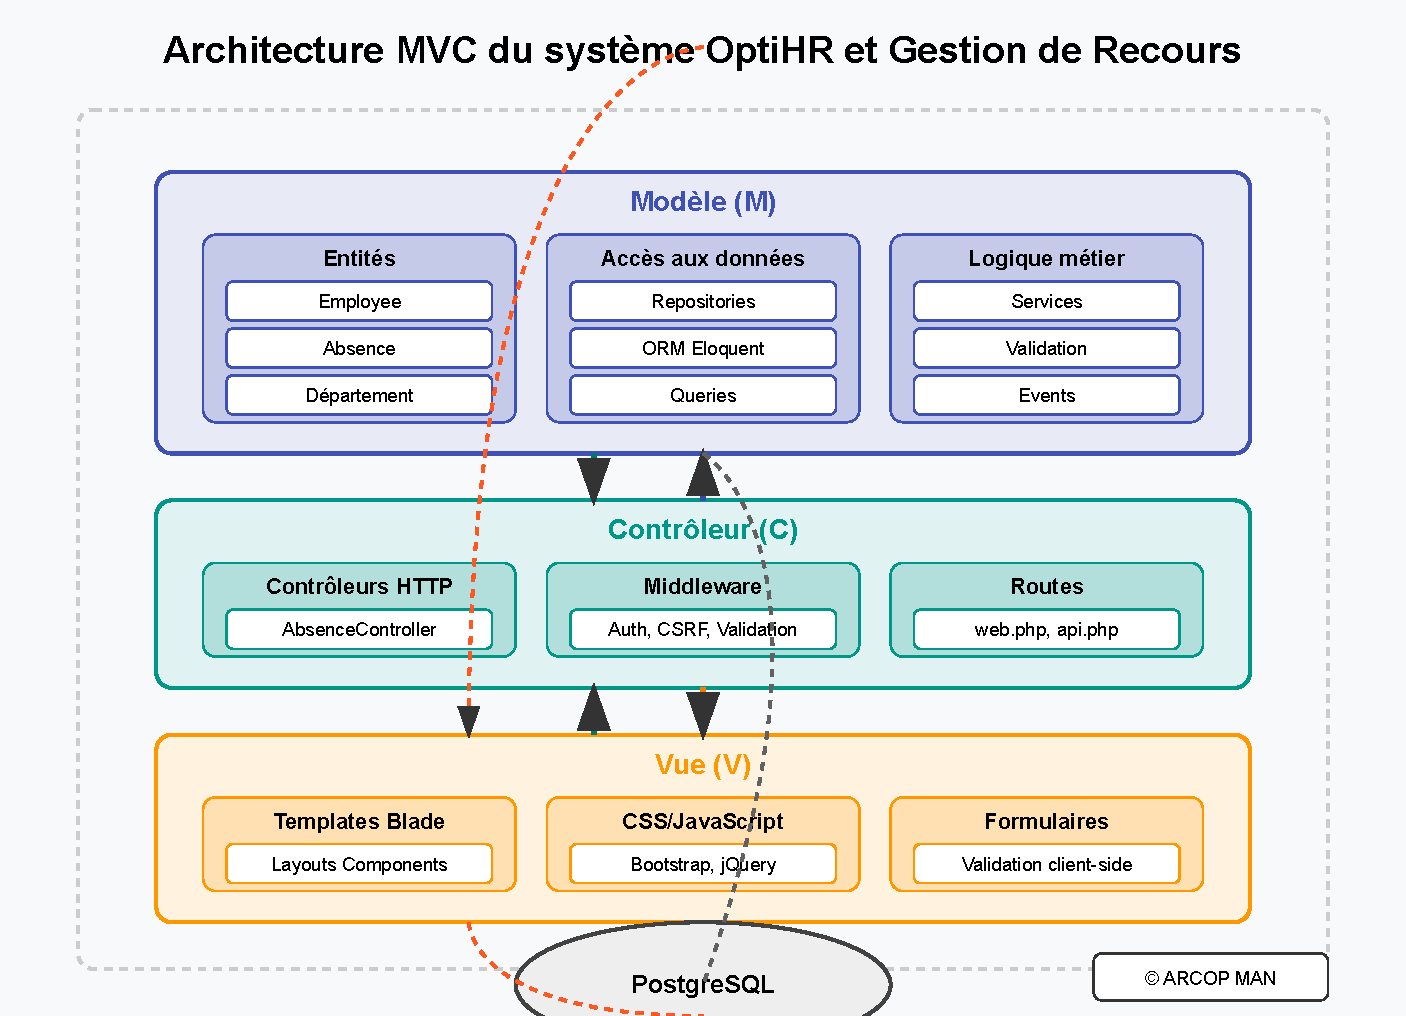
\includegraphics[width=0.9\textwidth]{images/diagrammes/architecture/architecture-couches.pdf}
    \caption{Architecture en couches du système OptiHR}
    \label{fig:architecture_couches}
\end{figure}

La figure \ref{fig:architecture_couches} illustre comment les différentes couches interagissent entre elles, avec un flux de données descendant pour les requêtes et ascendant pour les réponses. Les flèches représentent les dépendances entre les composants.

\subsection{Découpage modulaire du système}
Pour favoriser la maintenabilité et l'évolutivité, le système OptiHR est conçu selon une approche 
modulaire qui sépare les différentes préoccupations fonctionnelles:

\begin{enumerate}
    \item \textbf{Module d'authentification et autorisations}: Gestion des utilisateurs, des rôles et des permissions.
    \item \textbf{Module GRH}: Gestion des employés, des départements et de la documentation.
    \item \textbf{Module de gestion des absences}: Demandes de congés, workflow d'approbation et suivi.
    \item \textbf{Module de notifications}: Alertes système, notifications par email et notes de service.
    \item \textbf{Module documentaire}: Bulletins de paie, documents administratifs et archivage.
\end{enumerate}

\begin{figure}[H]
    \centering
    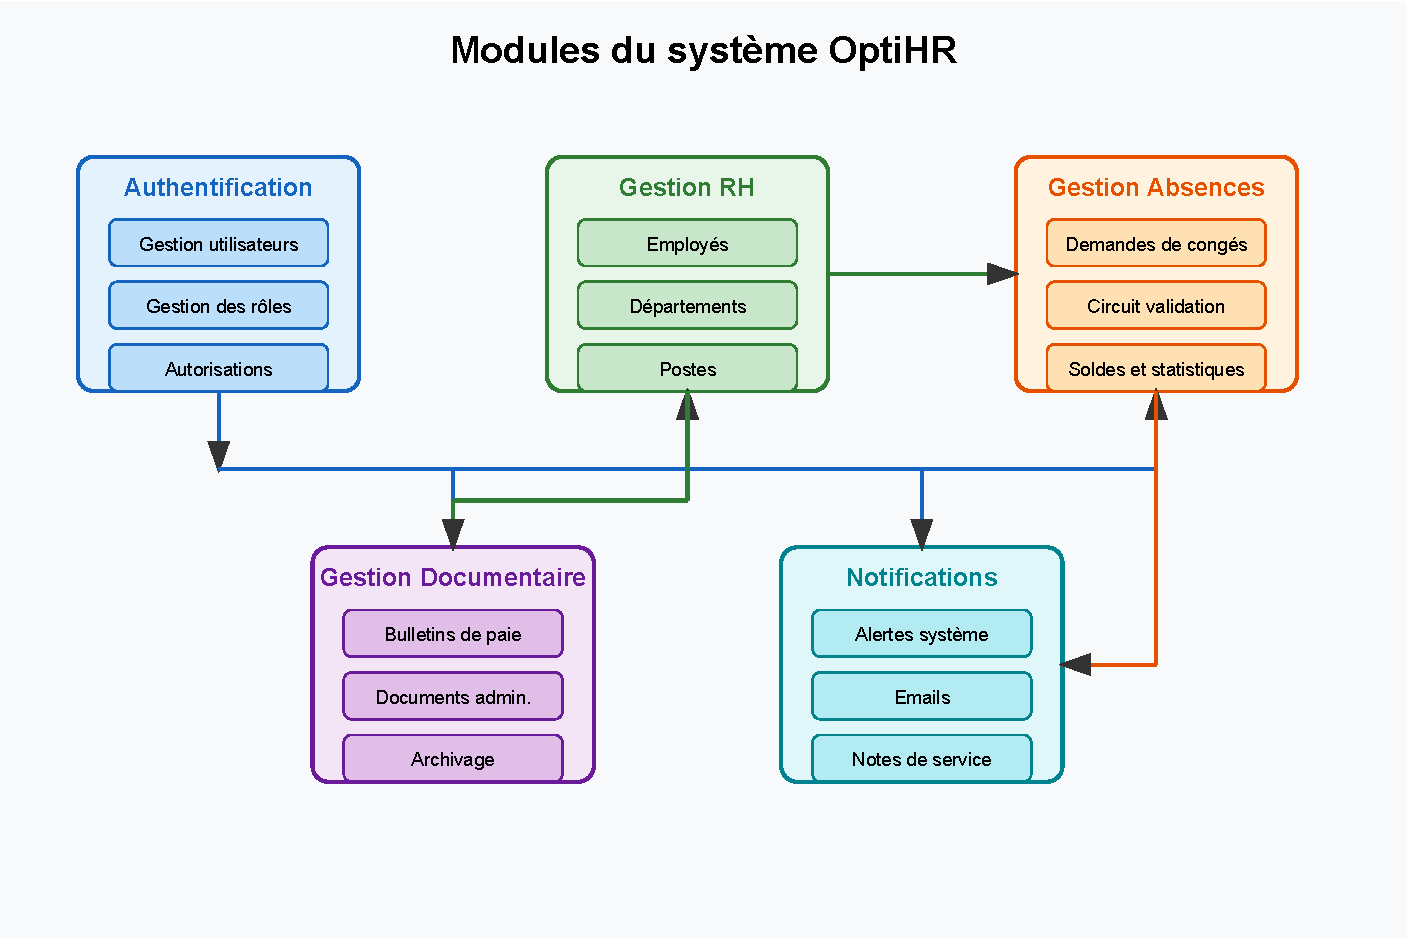
\includegraphics[width=0.9\textwidth]{images/diagrammes/architecture/modules-systeme.pdf}
    \caption{Organisation modulaire du système OptiHR}
    \label{fig:modules_systeme}
\end{figure}

Cette organisation modulaire, illustrée dans la figure \ref{fig:modules_systeme}, permet d'isoler les fonctionnalités 
et de faciliter les évolutions futures du système en minimisant les impacts entre modules.

\subsection{Flux de données et interactions}
Les interactions entre les composants suivent un flux standardisé qui garantit la cohérence des opérations
et facilite le débogage:

\begin{figure}[H]
    \centering
    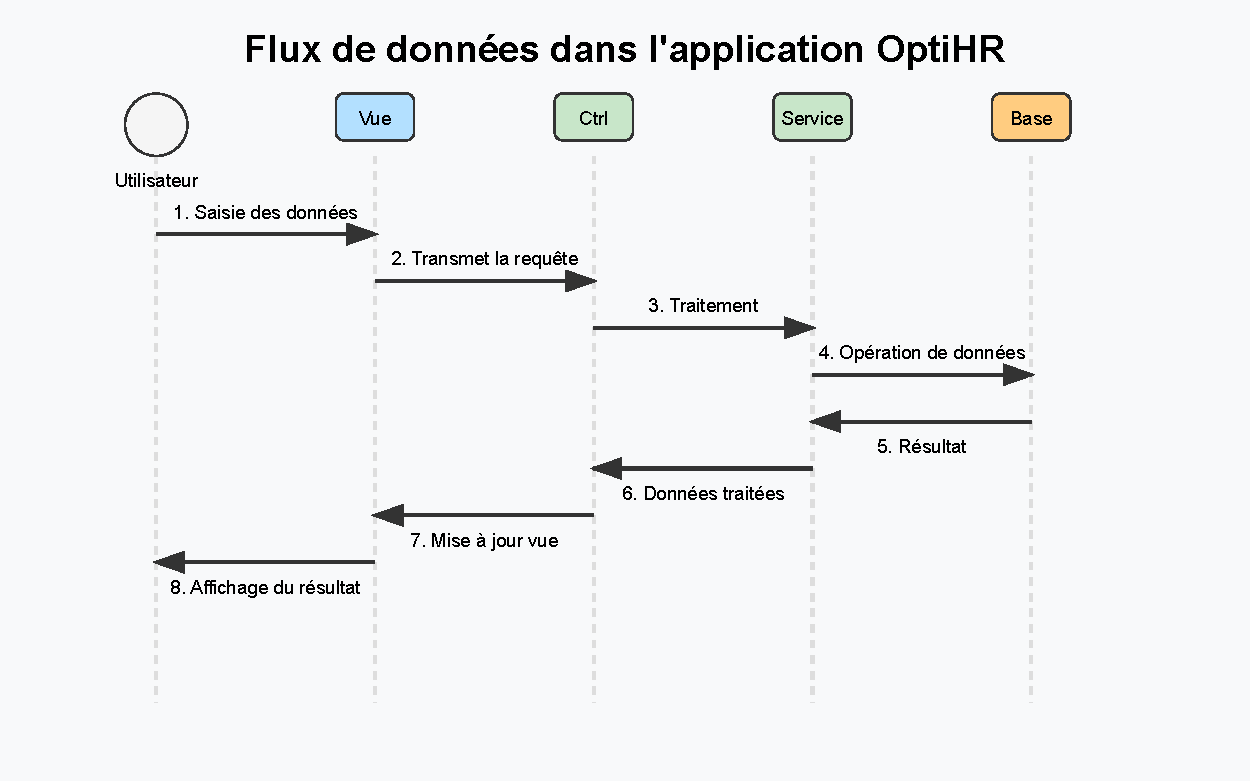
\includegraphics[width=0.9\textwidth]{images/diagrammes/architecture/flux-donnees.pdf}
    \caption{Flux de données dans l'application OptiHR}
    \label{fig:flux_donnees}
\end{figure}

Le diagramme de séquence (figure \ref{fig:flux_donnees}) détaille le parcours d'une requête typique à travers les différentes couches du système:

\begin{enumerate}
    \item L'utilisateur interagit avec l'interface (Vue)
    \item Les requêtes sont acheminées vers le Contrôleur approprié
    \item Le Contrôleur délègue le traitement aux Services
    \item Les Services manipulent les données via le Modèle
    \item Le Modèle interagit avec la base de données
    \item Les données sont remontées à travers les couches
    \item L'interface est mise à jour avec les résultats
    \item Le résultat final est affiché à l'utilisateur
\end{enumerate}


\section{Modélisation des données}

\subsection{Dictionnaire de données}
Le dictionnaire de données ci-dessous détaille les structures de stockage avec leurs attributs, 
types, contraintes et descriptions. Cette documentation précise garantit l'intégrité et 
la cohérence des données manipulées par le système.

\renewcommand{\arraystretch}{1.3} % Améliore l'espacement du tableau

\begin{longtable}{|p{2.5cm}|p{3cm}|p{3cm}|p{3cm}|p{3cm}|}
    \hline
    \textbf{Table} & \textbf{Attribut} & \textbf{Type SQL} & \textbf{Contrainte} & \textbf{Description} \\
    \hline
    \endfirsthead

    \hline
    \textbf{Table} & \textbf{Attribut} & \textbf{Type SQL} & \textbf{Contrainte} & \textbf{Description} \\
    \hline
    \endhead

    % User
    \multirow{5}{*}{\textbf{User}} & id & INT & PK, AUTO\_INCREMENT & Identifiant unique \\
    \cline{2-5}
    & username & VARCHAR(50) & NOT NULL, UNIQUE & Nom d'utilisateur \\
    \cline{2-5}
    & password & VARCHAR(255) & NOT NULL & Mot de passe haché \\
    \cline{2-5}
    & active & BOOLEAN & NOT NULL, DEFAULT TRUE & Statut du compte \\
    \cline{2-5}
    & employee\_id & INT & FK(Employee.id) & Référence à l'employé \\
    \hline

    % Employee
    \multirow{12}{*}{\textbf{Employee}} & id & INT & PK, AUTO\_INCREMENT & Identifiant unique \\
    \cline{2-5}
    & first\_name & VARCHAR(50) & NOT NULL & Prénom \\
    \cline{2-5}
    & last\_name & VARCHAR(50) & NOT NULL & Nom de famille \\
    \cline{2-5}
    & phone\_number & VARCHAR(20) & NULL & Numéro de téléphone \\
    \cline{2-5}
    & email & VARCHAR(100) & NOT NULL, UNIQUE & Adresse email \\
    \cline{2-5}
    & address1 & VARCHAR(255) & NULL & Adresse principale \\
    \cline{2-5}
    & address2 & VARCHAR(255) & NULL & Adresse secondaire \\
    \cline{2-5}
    & city & VARCHAR(50) & NULL & Ville \\
    \cline{2-5}
    & country & VARCHAR(50) & NULL & Pays \\
    \cline{2-5}
    & state & VARCHAR(50) & NULL & Région ou état \\
    \cline{2-5}
    & bank\_name & VARCHAR(100) & NULL & Nom de la banque \\
    \cline{2-5}
    & rib & VARCHAR(50) & NULL & RIB \\
    \cline{2-5}
    & department\_id & INT & FK(Department.id) & Département \\
    \hline

    % Department
    \multirow{3}{*}{\textbf{Department}} & id & INT & PK, AUTO\_INCREMENT & Identifiant unique \\
    \cline{2-5}
    & name & VARCHAR(100) & NOT NULL, UNIQUE & Nom du département \\
    \cline{2-5}
    & director\_id & INT & FK(Employee.id), NULL & Directeur \\
    \hline

    % Role
    \multirow{2}{*}{\textbf{Role}} & id & INT & PK, AUTO\_INCREMENT & Identifiant unique \\
    \cline{2-5}
    & name & VARCHAR(50) & NOT NULL, UNIQUE & Nom du rôle \\
    \hline

    % Permission
    \multirow{2}{*}{\textbf{Permission}} & id & INT & PK, AUTO\_INCREMENT & Identifiant unique \\
    \cline{2-5}
    & name & VARCHAR(50) & NOT NULL, UNIQUE & Nom de la permission \\
    \hline

    % Role_Permission
    \multirow{2}{*}{\textbf{Role\_Permission}} & role\_id & INT & PK, FK(Role.id) & Référence au rôle \\
    \cline{2-5}
    & permission\_id & INT & PK, FK(Permission.id) & Référence à la permission \\
    \hline

    % User_Role
    \multirow{2}{*}{\textbf{User\_Role}} & user\_id & INT & PK, FK(User.id) & Référence à l'utilisateur \\
    \cline{2-5}
    & role\_id & INT & PK, FK(Role.id) & Référence au rôle \\
    \hline

    % File
    \multirow{6}{*}{\textbf{File}} & id & INT & PK, AUTO\_INCREMENT & Identifiant unique \\
    \cline{2-5}
    & name & VARCHAR(255) & NOT NULL & Nom du fichier \\
    \cline{2-5}
    & url & VARCHAR(255) & NOT NULL & URL du fichier \\
    \cline{2-5}
    & mime\_type & VARCHAR(100) & NOT NULL & Type MIME \\
    \cline{2-5}
    & path & VARCHAR(255) & NOT NULL & Chemin d'accès \\
    \cline{2-5}
    & upload\_date & DATETIME & NOT NULL & Date d'upload \\
    \cline{2-5}
    & employee\_id & INT & FK(Employee.id) & Propriétaire \\
    \hline

    % Duty
    \multirow{5}{*}{\textbf{Duty}} & id & INT & PK, AUTO\_INCREMENT & Identifiant unique \\
    \cline{2-5}
    & duration & VARCHAR(50) & NOT NULL & Durée de la mission \\
    \cline{2-5}
    & begin\_date & DATE & NOT NULL & Date de début \\
    \cline{2-5}
    & type & VARCHAR(50) & NOT NULL & Type de mission \\
    \cline{2-5}
    & etat & VARCHAR(50) & NOT NULL & État de la mission \\
    \cline{2-5}
    & employee\_id & INT & FK(Employee.id) & Employé concerné \\
    \hline

    % Job
    \multirow{3}{*}{\textbf{Job}} & id & INT & PK, AUTO\_INCREMENT & Identifiant unique \\
    \cline{2-5}
    & title & VARCHAR(100) & NOT NULL & Intitulé du poste \\
    \cline{2-5}
    & supervisor\_id & INT & FK(Job.id), NULL & Poste supérieur \\
    \hline

    % Employee_Job
    \multirow{2}{*}{\textbf{Employee\_Job}} & employee\_id & INT & PK, FK(Employee.id) & Référence à l'employé \\
    \cline{2-5}
    & job\_id & INT & PK, FK(Job.id) & Référence au poste \\
    \hline

    % Absence
    \multirow{12}{*}{\textbf{Absence}} & id & INT & PK, AUTO\_INCREMENT & Identifiant unique \\
    \cline{2-5}
    & day\_requested & INT & NOT NULL & Jours demandés \\
    \cline{2-5}
    & start\_date & DATE & NOT NULL & Date de début \\
    \cline{2-5}
    & end\_date & DATE & NOT NULL & Date de fin \\
    \cline{2-5}
    & address & VARCHAR(255) & NULL & Adresse durant l'absence \\
    \cline{2-5}
    & date\_of\_application & DATE & NOT NULL & Date de la demande \\
    \cline{2-5}
    & status & VARCHAR(20) & NOT NULL & Statut de l'absence \\
    \cline{2-5}
    & date\_of\_approval & DATE & NULL & Date d'approbation \\
    \cline{2-5}
    & type\_of\_absence & VARCHAR(50) & NOT NULL & Type d'absence \\
    \cline{2-5}
    & reasons & TEXT & NULL & Raisons de l'absence \\
    \cline{2-5}
    & proof & VARCHAR(255) & NULL & Justificatif \\
    \cline{2-5}
    & comment & TEXT & NULL & Commentaire \\
    \cline{2-5}
    & employee\_id & INT & FK(Employee.id) & Employé concerné \\
    \hline

    % Note
    \multirow{4}{*}{\textbf{Note}} & id & INT & PK, AUTO\_INCREMENT & Identifiant unique \\
    \cline{2-5}
    & message & TEXT & NOT NULL & Contenu de la note \\
    \cline{2-5}
    & file & VARCHAR(255) & NULL & Fichier joint \\
    \cline{2-5}
    & publish\_date & DATETIME & NOT NULL & Date de publication \\
    \cline{2-5}
    & author\_id & INT & FK(Employee.id) & Auteur de la note \\
    \hline

    % Decision
    \multirow{5}{*}{\textbf{Decision}} & id & INT & PK, AUTO\_INCREMENT & Identifiant unique \\
    \cline{2-5}
    & number & VARCHAR(20) & NOT NULL & Numéro de décision \\
    \cline{2-5}
    & year & VARCHAR(4) & NOT NULL & Année de la décision \\
    \cline{2-5}
    & date & DATE & NOT NULL & Date de la décision \\
    \cline{2-5}
    & content & TEXT & NOT NULL & Contenu de la décision \\
    \hline

    % Image
    \multirow{6}{*}{\textbf{Image}} & id & INT & PK, AUTO\_INCREMENT & Identifiant unique \\
    \cline{2-5}
    & name & VARCHAR(255) & NOT NULL & Nom de l'image \\
    \cline{2-5}
    & url & VARCHAR(255) & NOT NULL & URL de l'image \\
    \cline{2-5}
    & mime\_type & VARCHAR(100) & NOT NULL & Type MIME \\
    \cline{2-5}
    & path & VARCHAR(255) & NOT NULL & Chemin d'accès \\
    \cline{2-5}
    & entity\_id & INT & NOT NULL & ID entité associée \\
    \cline{2-5}
    & entity\_type & VARCHAR(50) & NOT NULL & Type entité associée \\
    \hline
\end{longtable}
\begin{table}[H]
    \centering
    \caption{Dictionnaire des données amélioré}
    \label{tab:table_dictionnaire_data_ameliore}
\end{table}

\section{Modélisation objet}

\subsection{Diagramme de classes}
Le diagramme de classes constitue la représentation structurelle du système OptiHR. Il modélise les entités du domaine, leurs attributs et les relations qu'elles entretiennent entre elles. Cette modélisation répond aux besoins métier identifiés lors de la phase d'analyse et traduit fidèlement les processus de gestion des ressources humaines de l'ARCOP.

\begin{figure}[H]
    \centering
    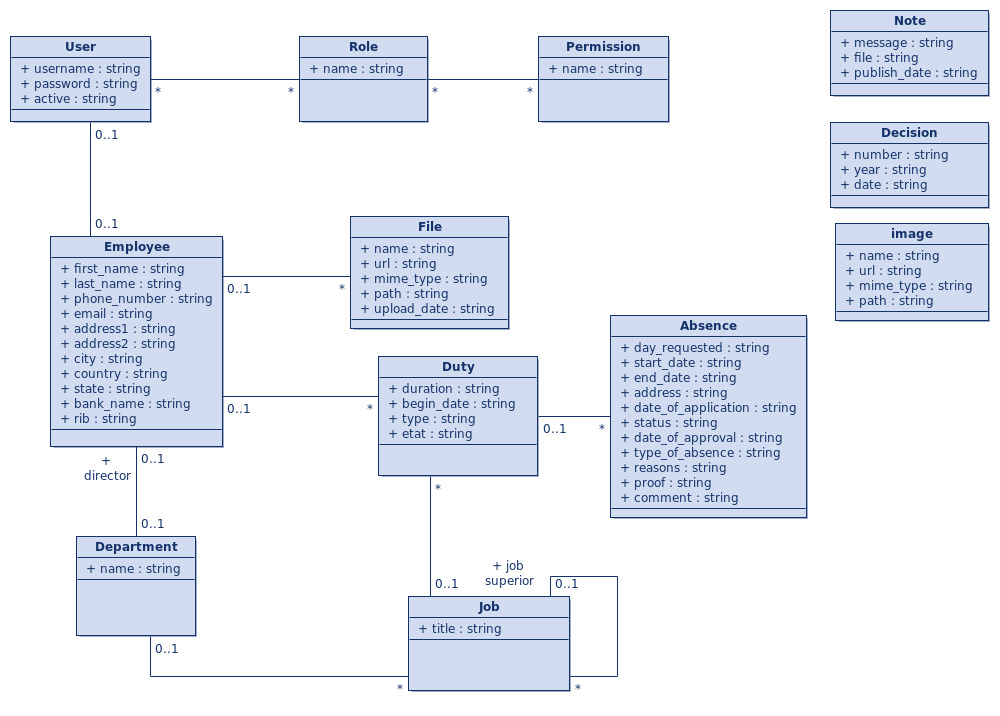
\includegraphics[width=\textwidth]{images/diagrammes/class/diagramme.jpeg}
    \caption{Diagramme de classes amélioré du système OptiHR}
    \label{fig:class_diagram_improved}
\end{figure}

La figure \ref{fig:class_diagram_improved} présente le diagramme de classes complet du système. Pour faciliter la compréhension, les entités sont regroupées par domaine fonctionnel:

\begin{itemize}
    \item \textbf{Domaine Utilisateur}: Gestion des accès et des permissions (User, Role, Permission)
    \item \textbf{Domaine Ressources Humaines}: Organisation et employés (Employee, Department, Job)
    \item \textbf{Domaine Opérationnel}: Activités et processus métier (Absence, Duty)
    \item \textbf{Domaine Documentaire}: Gestion des documents et médias (File, Image, Note, Decision)
\end{itemize}

\subsection{Relations et multiplicités}
Les relations entre les classes représentent les associations fonctionnelles au sein du système. Chaque relation est caractérisée par sa nature (association, composition, agrégation) et sa multiplicité, qui définit le nombre d'instances impliquées.

\begin{enumerate}
    \item \textbf{Employee - Department} (n:1): Un employé appartient à un seul département, tandis qu'un département peut regrouper plusieurs employés.
    
    \item \textbf{Employee - Job} (n:m): Un employé peut occuper plusieurs postes au cours de sa carrière, et un même poste peut être occupé par différents employés successivement. Cette relation est matérialisée par l'association \texttt{Employee\_Job}.
    
    \item \textbf{Employee - Absence} (1:n): Un employé peut enregistrer plusieurs absences, mais chaque absence est associée à un seul employé.
    
    \item \textbf{User - Employee} (1:1): Chaque utilisateur du système est associé à un employé spécifique, établissant ainsi le lien entre l'identité numérique et la personne physique.
    
    \item \textbf{User - Role} (n:m): Un utilisateur peut avoir plusieurs rôles, et un même rôle peut être attribué à plusieurs utilisateurs. Cette relation est matérialisée par l'association \texttt{User\_Role}.
    
    \item \textbf{Role - Permission} (n:m): Un rôle regroupe plusieurs permissions, et une même permission peut appartenir à différents rôles. Cette relation est matérialisée par l'association \texttt{Role\_Permission}.
    
    \item \textbf{Job - Job} (n:1): Relation réflexive représentant la hiérarchie des postes. Un poste peut avoir un poste supérieur (\texttt{supervisor\_id}), créant ainsi la structure hiérarchique.
    
    \item \textbf{Department - Employee} (1:1): Relation particulière identifiant le directeur du département parmi ses employés.
\end{enumerate}

\section{Technologies et outils}
Les outils et technologies suivants ont été utilisés pour la conception du
projet \textbf{OptiHR}. Chaque outil est accompagné d'une image et d'une
description détaillée.

\vspace{1cm} % Ajoute un espace vertical

\renewcommand{\arraystretch}{1.5} % Espacement entre les lignes du tableau

\begin{center}
    \begin{table}[H]  % Environnement table pour être listé dans la liste des tableaux
       

        \begin{tabular}{|m{4cm}|m{10cm}|}
            \hline
            \textbf{Technologie}                                 & \textbf{Description}                                                                                                                                                                             \\
            \hline

            
\includegraphics[width=3cm]{images/logo/uml.png}     & \textbf{UML} : Utilisé pour la modélisation des systèmes et la conception des structures du projet. Il permet de représenter graphiquement les différentes interactions et processus du système. \\
            \hline

            
\includegraphics[width=3cm]{images/logo/modelio.png} & \textbf{Modelio} : Outil de modélisation UML permettant de créer des diagrammes tels que les diagrammes de classes, de séquence et d'activités.                                                  \\
            \hline

        \end{tabular}
        % \centering
        \caption{Tableau des technologies et outils utilisés pour la conception} % La légende du tableau
        \label{tab:technos_conception} % Étiquette pour référence
    \end{table}
\end{center}

\section{Conclusion}
La phase de conception pose les bases essentielles du projet en structurant
l'architecture et en précisant les technologies et les modèles de données
adoptés. Une conception rigoureuse garantit un développement fluide et
efficace, tout en assurant la maintenance et l'évolutivité du système sur le
long terme.

\clearpage